\newpage

\begin{lstlisting}[language=JuliaLocal, style=julia]
using PlutoUI
\end{lstlisting}

\begin{lstlisting}[language=JuliaLocal, style=julia]
begin
	using Plots
	y(x) = sin(x)
	plot(y,
		color=:blue)
end
\end{lstlisting}

\begin{figure}[H]
	\centering
	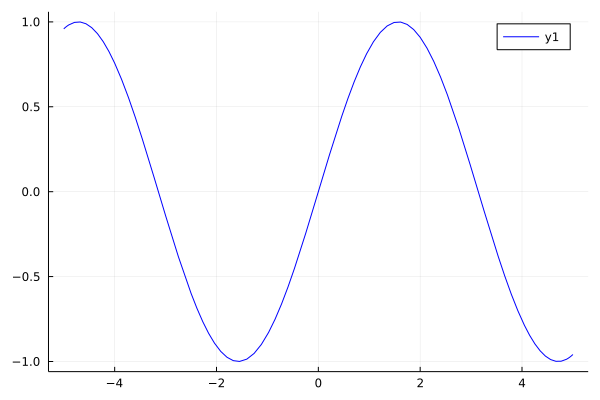
\includegraphics[width=0.8\textwidth]{./figures/examplepluto_figure1.png}
	\label{fig:examplepluto_figure1.png}

\end{figure}

\begin{lstlisting}[language=JuliaLocal, style=julia]
A = [10,10,10]
\end{lstlisting}

\begin{verbatim}
3-element Vector{Int64}:
 10
 10
 10
\end{verbatim}

\begin{lstlisting}[language=JuliaLocal, style=julia]
x = rand(10);
\end{lstlisting}

\begin{lstlisting}[language=JuliaLocal, style=julia]
x .+ 1
\end{lstlisting}

\begin{verbatim}
10-element Vector{Float64}:
 1.0837366758576608
 1.1482332607517722
 1.2059359955640943
 1.045109060552612
 1.8264439852727543
 1.3772653850174172
 1.2022775461602926
 1.5779963285186436
 1.3065782691415349
 1.042751787519958
\end{verbatim}

\begin{lstlisting}[language=JuliaLocal, style=julia]
set_theme!(theme_ggplot2())
\end{lstlisting}

\begin{lstlisting}[language=JuliaLocal, style=julia]
Makie.plot(x)
\end{lstlisting}

\begin{figure}[H]
	\centering
	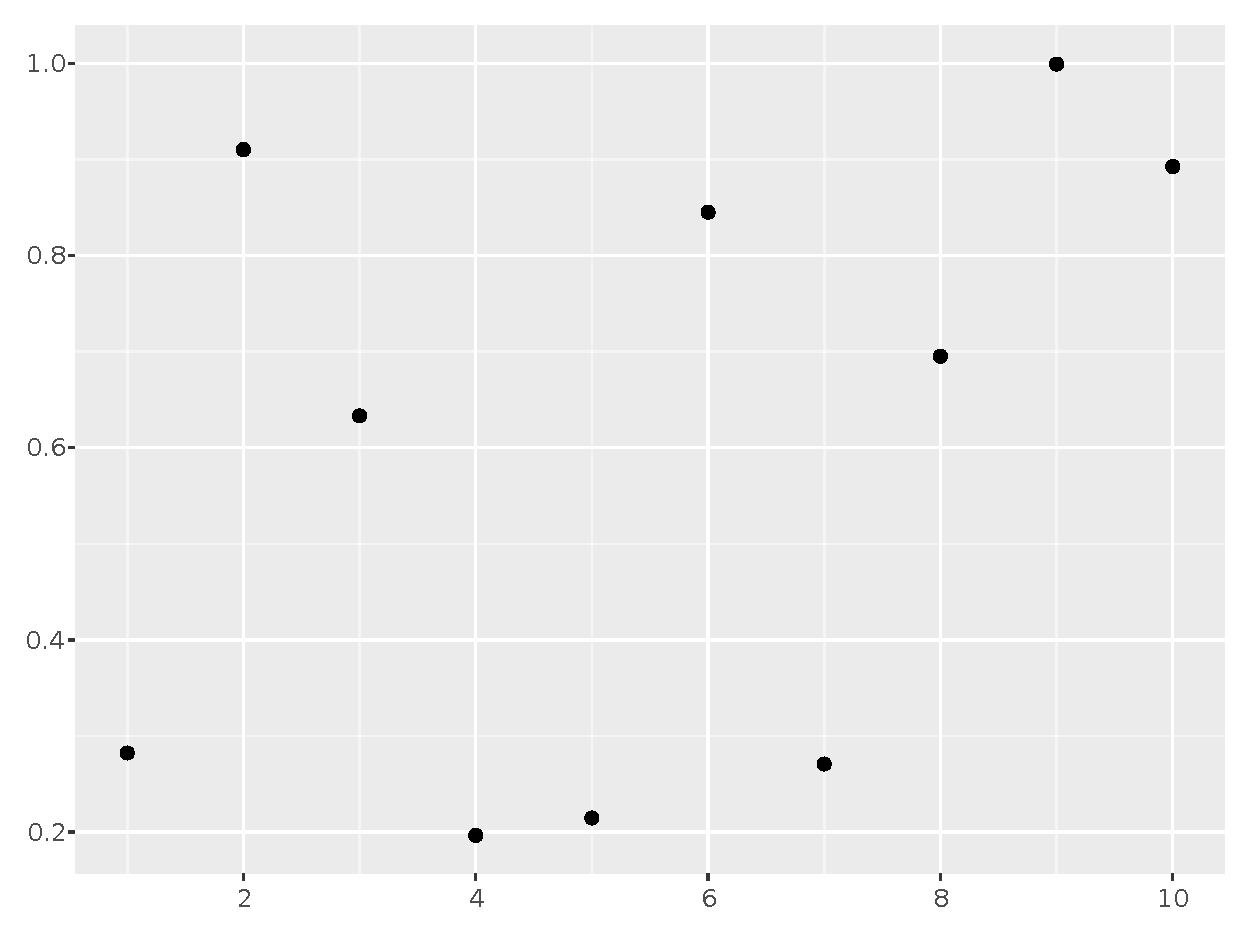
\includegraphics[width=0.8\textwidth]{./figures/examplepluto_figure2.pdf}
	\label{fig:examplepluto_figure2.pdf}

\end{figure}

\begin{lstlisting}[language=JuliaLocal, style=julia]
PlutoUI.LocalResource(figurepath)
\end{lstlisting}

\begin{figure}[H]
	\centering
	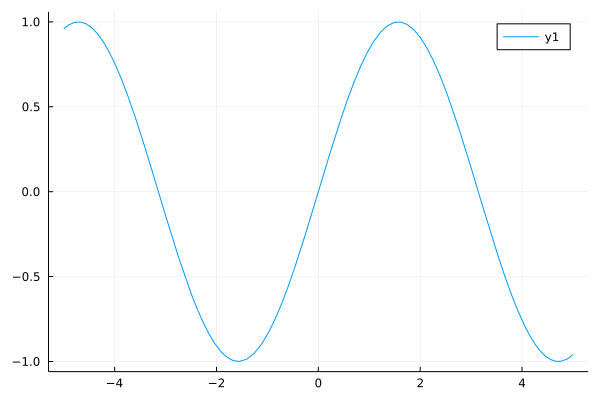
\includegraphics[width=0.8\textwidth]{/home/davibarreira/MEGA/EMAp/PlutoLatexConverter.jl/example/plotexample.png}
	\label{fig:/home/davibarreira/MEGA/EMAp/PlutoLatexConverter.jl/example/plotexample.png}

\end{figure}
